

\documentclass[12pt, a4paper]{article}


\usepackage{fancyhdr, enumerate}
\usepackage{amssymb}
\usepackage{geometry, amsmath, amsfonts, float, graphicx}
\usepackage{gensymb}
\usepackage{hyperref, listings}
\usepackage{matlab-prettifier}
\usepackage{caption}
\geometry{
	top=0.9in,           
	inner=0.6in,
	outer=0.6in,
	bottom=2in,
	tmargin= 10ex,       
	headsep=0.6cm,          
}
\pagestyle{fancy}

\fancyhead{}
\fancyfoot{}

\fancyhead[L]{Bioen 316 AC \\Homework 3\\ April 24, 2019}
\fancyhead[R]{Skyler Hallinan\\ hallisky@uw.edu \\ 1732227}

\lstMakeShortInline[style=Matlab-editor]"
\begin{document}
\vspace*{-3mm}
\section*{Problem}
Flex sensors are variable resistors that change resistance according to how much they are
bent, so they are good candidates for a voltage divider or bridge circuit. One application is
to attach a flex sensor on the back of a finger in a prosthetic hand to measure how much the
hand is closed. Let’s assume that the hand can open flat to $\theta = 0 \degree$ and close to a 90$\degree$ bend,
with a resting angle of $\theta = 30 \degree$. The FlexSensor by Spectra Symbol has a resistance of 25 k$\Omega$
when flat and 125 k$\Omega$ when bent 90$\degree$. A simple, but not very accurate, mathematical model
of the relationship is $R_{FS}(\theta) = 25e^{0.012\theta}$ k$\Omega$ with $\theta$ in degrees. This function is non-linear,
but it can be linearized around 30$\degree$ by using the first two terms in the Taylor series: $R(\theta) \approx R_{FS}(30 \degree) + \Delta \theta \cdot \frac{dR}{d\theta} |_{\theta = 30}$. Note that $\Delta \theta = \theta -30 \degree$
\begin{enumerate}

\item Linearize the original $R_{FS}(\theta)$ function around $30 \degree$ to create a new, approximate $R(\theta)$ \\ \\
\textbf{Answer: } \\
We can linearize the function using the first two terms in the Taylor Series: 
\begin{align*}
R(\theta) &\approx R_{FS}(30 \degree) + \Delta \theta \cdot \frac{dR}{d\theta} |_{\theta = 30} &\Delta \theta = \theta -30 \degree, \quad R_{FS} = 25e^{0.012 \theta} \\
&\approx 25 e^{0.012 \cdot 30} + (\theta - 30) 0.3 e^{0.012 \cdot 30} \\
&\approx 16e^{0.36} + 0.3 e^{0.36} \theta \\
& \approx e^{0.36} [16 + 0.3 \theta]	\ k\Omega
\end{align*}

\item Show that you can use a simple voltage divider to achieve an output of 2.0 V when the bend angle is 30 $\degree$. To do this, apply a supply voltage of +5 V across three components in series: the flex sensor, a fixed resistance $R_0$, and a potentiometer of 10 k$\Omega$ or less. Arrange the circuit so the output voltage increases when the bend angle increases; whether it increases or decreases depends on whether the FlexSensor is connected to ground or to the 5 V supply. For $R_0$, use any $\frac{1}{4}-W$ resistors available in standard values, which are
shown in the table on the following page. In addition, all resistors are subject to error from
the manufacturing process, and you can adjust the potentiometer to accommodate this
error. Your analysis should show that, even with the manufacturing error and a limited
choice of resistor values, your potentiometer’s range is big enough to achieve the value of
$R_0$ that you need.\\ \\
\textbf{Answer: } \\
Since our circuit is in series, the total resistance of the circuit will equal the sum of the resistance of each component in the circuit. We calculate the following (resistance units in k$\Omega$): \begin{align*}
V &= IR, \quad R_{FS}(\theta) = e^{0.36} [16 + 0.3 \theta] \ k\Omega \quad &\text{Ohm's Law, Linearization} \\
R_{FS}(30) \approx 35.83 \ k\Omega, \quad &R_{P} \leq 10 \Rightarrow R_P = 5 \ k\Omega, \quad R_0 = ? &\text{Set $R_{P}$ = 5 k$\Omega$}\\ 
R_{total} = R_{FS} + R_{P} + R_0 &\approx 40.83 + R_0 \ k\Omega, \quad V_{input} = 5 V\\
5 &= I (40.83 + R_0) \quad  &\text{Substitute $V_{input}$ and $R_{total}$}\\
\end{align*}
We assumed our potentiometer voltage to be 5V, in the middle between the limits of 0 and 10. This allows us to increase or decrease it depending on the error of the fixed resistance resistor; we should be able to increase or decrease the potentiometer resistance to keep the total resistance in the circuit constant. In addition, we used the properties of resistors in series to find the total resistance in the circuit and write a relation between the current, resistance, and voltage. \\ \\
We also see that the voltage output should increase as the angle and therefore the resistance of the flex sensor increases. The flex sensor will have increasing resistance as its bend angle increases, while the other voltages and the other resistances stay constant: this means that the ratio $\frac{R_{FS}}{R_{total}}$ will increase when $R_{FS}$ increases. Since $V = IR$ and $V_{output} = V_{input} \frac{R_{item}}{R_{total}}$, where $R_{item}$ is the resistance of the last element in the circuit, increasing the resistance of the flex sensor will increase the output voltage, only if the flex sensor is the last item in the series circuit: we must substitute $R_{FS}$ for the arbitrary $R_{item}$ (We note that the current $I$ is constant through this series circuit). This means that the flex sensor should be connected to the ground, so that our voltage drop in our last element (our voltage output) corresponds to the circuit element with a higher resistance at higher flex angles, which then in turn corresponds to higher voltage output at higher bend angles. \\ \\
Placing our flex sensor near the ground, at the end of the circuit, makes it so that our voltage out is directly related to the resistance of this flex sensor, as it is the last component of the circuit to have its voltage drop and $ V = IR$. Having the flex sensor at the end of the circuit ensures that it, with it's increasing resistance, it is responsible for the voltage out, which will now increase with increasing angle in the flex sensor. With these assumptions, we can set up another equation to solve for the current in the circuit (since it is constant throughout the circuit). \\ 
\begin{align*}
V = IR , \quad R_{FS} &= 35.83 \ k\Omega, \quad V_{output} = 2 V &\text{Ohm's Law, Constants}\\
2 &= I (35.83) &\text{$V_{output}$ and $R_{FS}$ substitution} \\
I &\approx 0.0558 \  mA\\
0.0558 &= \frac{5}{40.83 + R_0} &\text{Substitute $V_{input}$, $R_{total}$, and I into Ohm's Law}\\
R_0 &= \frac{5}{0.0558} - 40.83 \\ 
		&= 48.7757 \ k \Omega
\end{align*}
We see from the table that the closest resistance for our fixed resistor $R_0$ is 47 k$\Omega$. Since we want the sum of all three resistances to be constant, since $R_0$ is increased by $48.7757 - 47 = 1.7757$ k$\Omega$, we increase our $R_p$ by 1.7757 k$\Omega$ so that $R_{total} = R_{FS} + R_0 + R_P$ remains constant: 
\begin{align*}
R_{total} &= R_{FS} + (R_0 -1.7757) + (R_P+1.7757) \\
 &= R_{FS} + R_0 + R_P\\ 
 R_0 = 47\ k\Omega, \quad& R_P = 6.7757\ k\Omega
\end{align*}
Then, we draw a circuit diagram to demonstrate that the voltage drop is indeed 2V, with an input voltage of 5V: \\
\begin{figure}[h]
\centering
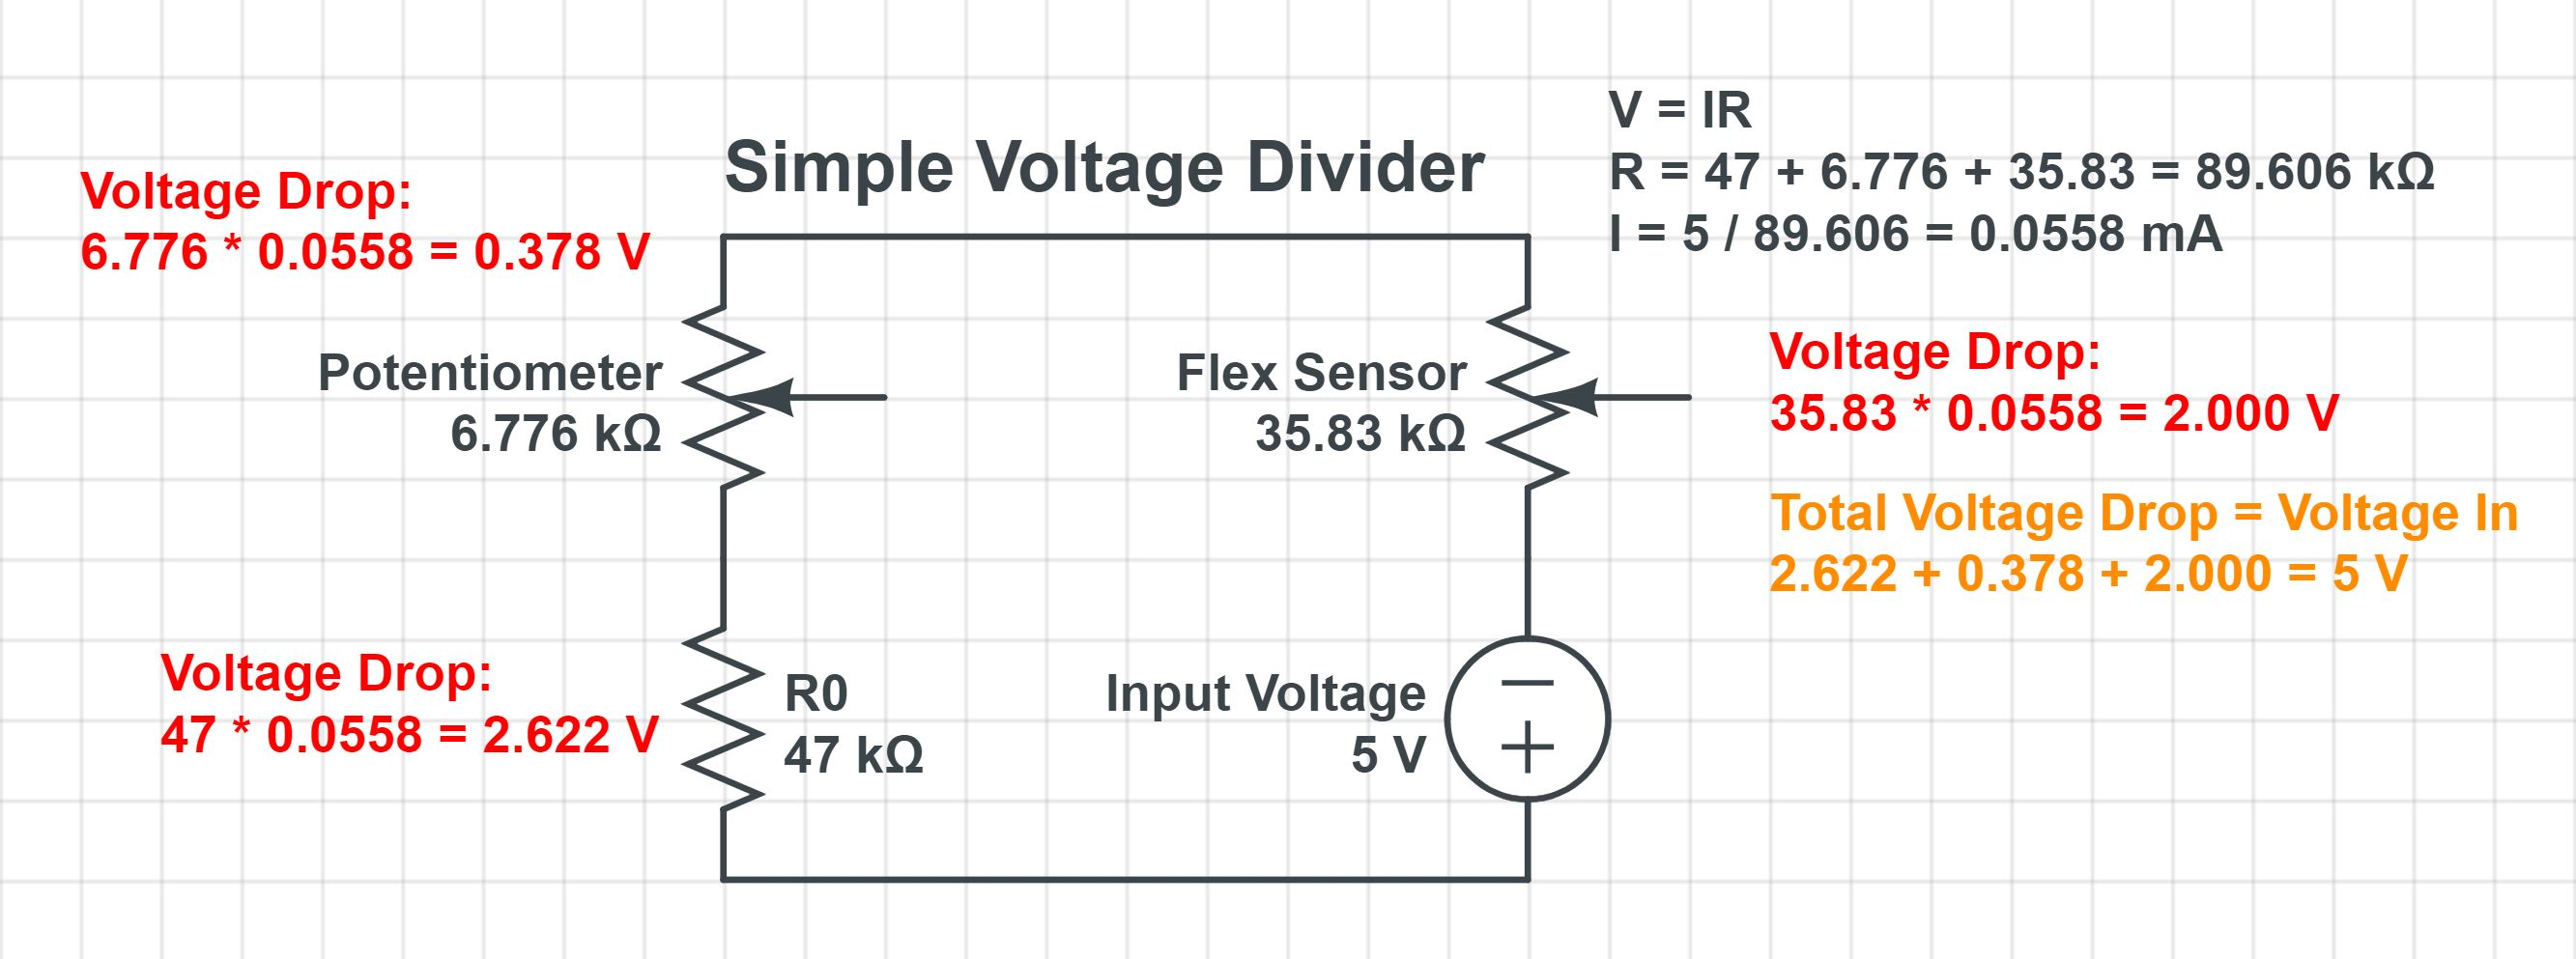
\includegraphics[width=1\textwidth]{samp6}
\caption{Circuit diagram for simple voltage divider with calculated values}
\end{figure}
\\
We see that our voltage output (represented by the voltage drop by the last component in the circuit, the flex sensor) is 2V with our calculated resistances for the other circuit components, and an input voltage of 5V. We also see that the total voltage drop around the circuit is 5V while the input voltage is 5V, which matches Kirckhoff's Rule, which states that around a loop, the voltage must sum to 0. \\ \\
Finally, one thing we must consider is error in our ordered $R_0$ resistor. Our $R_0$ can have up to a 5$\%$ error in the amount of resistance it has from the value stated. The potentiometer exists to offset this error by increasing/decreasing its own resistance based on the change in the $R_0$, therefore keeping the sum of all resistances constant. We see that our $R_0 = 47$  k$\Omega$, our $R_P = 6.7757$  k$\Omega$, and that our $R_P$ can be between 0 and 10  k$\Omega$. We also see the sum $R_0 + R_P = 53.7757$ k$\Omega$. The max error that we can achieve (5\%) of the $R_0$ is of $0.05 \cdot 47 =  \pm 2.35 \ k\Omega$, that is, we may receive a resistor $R_0$ with a resistance range between 44.65 and 49.35  k$\Omega$. However, we see that the potentiometer can remedy this. \\ \\
 If the error is at its maximum positive value, $+ 2.35$  k$\Omega$, and our $R_0$ has a resistance of 49.35 k$\Omega$, then we can decrease the $R_P$ by 2.35 k$\Omega$ to offset this; the new $R_P$ becomes 4.4257 k$\Omega$. This resistance is achievable by our potentiometer because it is between 0 and 10 (we don't consider $R_{FS}$ in these calculations because it is a constant). Therefore, we have proven that the potentiometer can remedy up to the maximum positive error in the $R_0$:
\begin{align*}
R_{total} &= (R_0 + 2.35) + (R_P - 2.35) + R_{FS} \\
R_{total}&= R_0 + R_P  + R_{FS}\\
R_0 = 49.35\ k\Omega, &\quad R_P = 4.4257\ k\Omega &0 < R_P \leq 10\ k\Omega
\end{align*}
Similarly, if the error is at its maximum negative value, $-2.35$ k$\Omega$, and our $R_0$ has a resistance of 44.65 k$\Omega$, we can \textbf{increase} the $R_P$ by 2.35 k$\Omega$ to offset this; the new $R_P$ becomes 9.1257 k$\Omega$. This resistance is also achievable by our potentiometer because it is greater than 0 and less than 10 k$\Omega$. Therefore, we have proven that the potentiometer can remedy up to the maximum negative error in the $R_0$:
\begin{align*}
R_{total} &= (R_0 - 2.35) + (R_P + 2.35) + R_{FS} \\
R_{total}&= R_0 + R_P  + R_{FS} \\
R_0 = 44.65 \ k\Omega, &\quad R_P = 9.1257\ k\Omega  &0 < R_P \leq 10\ k\Omega
\end{align*}
We have therefore demonstrated that we are able to achieve our desired total resistance sum, with $R_0 + R_P = 53. 7757$ k$\Omega$ and $R_{FS}$ being a constant, even with a 5$\%$ error in our expected $R_0$ value (of 47 k$\Omega$). We are able to do this by shifting our potentiometer to values between 0 and 10 to offset any error that may appear in our $R_0$.
\item Once you have set up your circuit to get an output of 2.0 V, determine the sensitivity
of this voltage divider circuit in volts/degree. Hint: The sensitivity is a rate of change, and
the slope or rate of change of a function can be found via its derivative. \\ \\
\textbf{Answer: } \\
The voltage output from our circuit can be determined from Ohm's Law, and is dependent on the total input voltage in the circuit, the total resistance (sum of resistance of the components in series), and the resistance of the final component (the flex sensor). To see the sensitivity of our output voltage, in voltage/degree, we must take the derivative of this voltage with respect to $\theta$. We can then substitute our $\theta = 30$ value to see sensitivity at a specific bend angle.
\begin{align*}
V_{input} &= IR_{total}, \quad V_{output} = IR_{FS} &\text{Ohm's Law} \\
\frac{V_{input}}{R_{total}} &= \frac{V_{output}}{R_{FS}} &\text{I is the same for both equations} \\
V_{output} &= \frac{V_{input} \cdot R_{FS}}{R_{total}} \\
 &= \frac{5 \cdot  e^{0.36} [16 + 0.3 \theta]}{47 + 6.7757 + e^{0.36} [16 + 0.3 \theta]} &\text{Substitute values}\\
&= \frac{114.67 + 2.15 \theta}{76.71 + 0.43\theta} \\
\frac{dV_{output}}{d\theta} &= \frac{2.15(76.71 + 0.43\theta) - 0.43(114.67 + 2.15 \theta)}{(76.71 + 0.43\theta)^2} &\text{Differentiate w.r.t. $\theta$}\\
&= \frac{115.62}{(76.71 + 0.43\theta)^2} \\
V'(30) &\approx 0.0144 \frac{volts}{degree}&\text{$\theta$ = 30 $\degree$}
\end{align*}
We see that at $\theta = 30 \degree$, we have a output voltage sensitivity of 0.0144 volts/degree.
\item Take the flex sensor out of the voltage divider and put it in a Wheatstone bridge,
replacing $R_2$ in the figure above. The two $R_1$’s should be equal, not adjustable, and within
10$\%$ of the flex sensor value; you may assume the $R_1$’s have zero error. $R_3$, which is the
sum of a fixed resistor plus 10 k$\Omega$ potentiometer, should match the flex sensor resistance at
30$\degree$. Once again, choose from among the available fixed resistor values. Show that your
circuit creates an output voltage difference of 0 V for any power supply voltage. \\ \\
\textbf{Answer: } \\
We set $R_3$ to be the flex sensor resistance at 30$\degree$, $R_{FS}(30) = R3 \approx$ 35.83 k$\Omega$ (we can assume that it has this uneven number because we have a potentiometer that can add voltage to a fixed resistance from the table). We also assume $\theta = 30 \degree$, and set the value of $R_2$, the component that represents our flex sensor, to $R_{FS}(30) = R2 \approx 35.83$ k$\Omega$. Finally, we see that since $R_1$ must be within 10 $\%$ of the flex sensor reistance which is currently 35.83 k$\Omega$, we see from the table that the $R_1 = 33$ k$\Omega$ (which is within 10$\%$ of 35.83). We then construct the following circuit diagram, arbitrarily setting voltage to 5V (we can use any positive voltage here). \\
\begin{figure}[h]
\centering
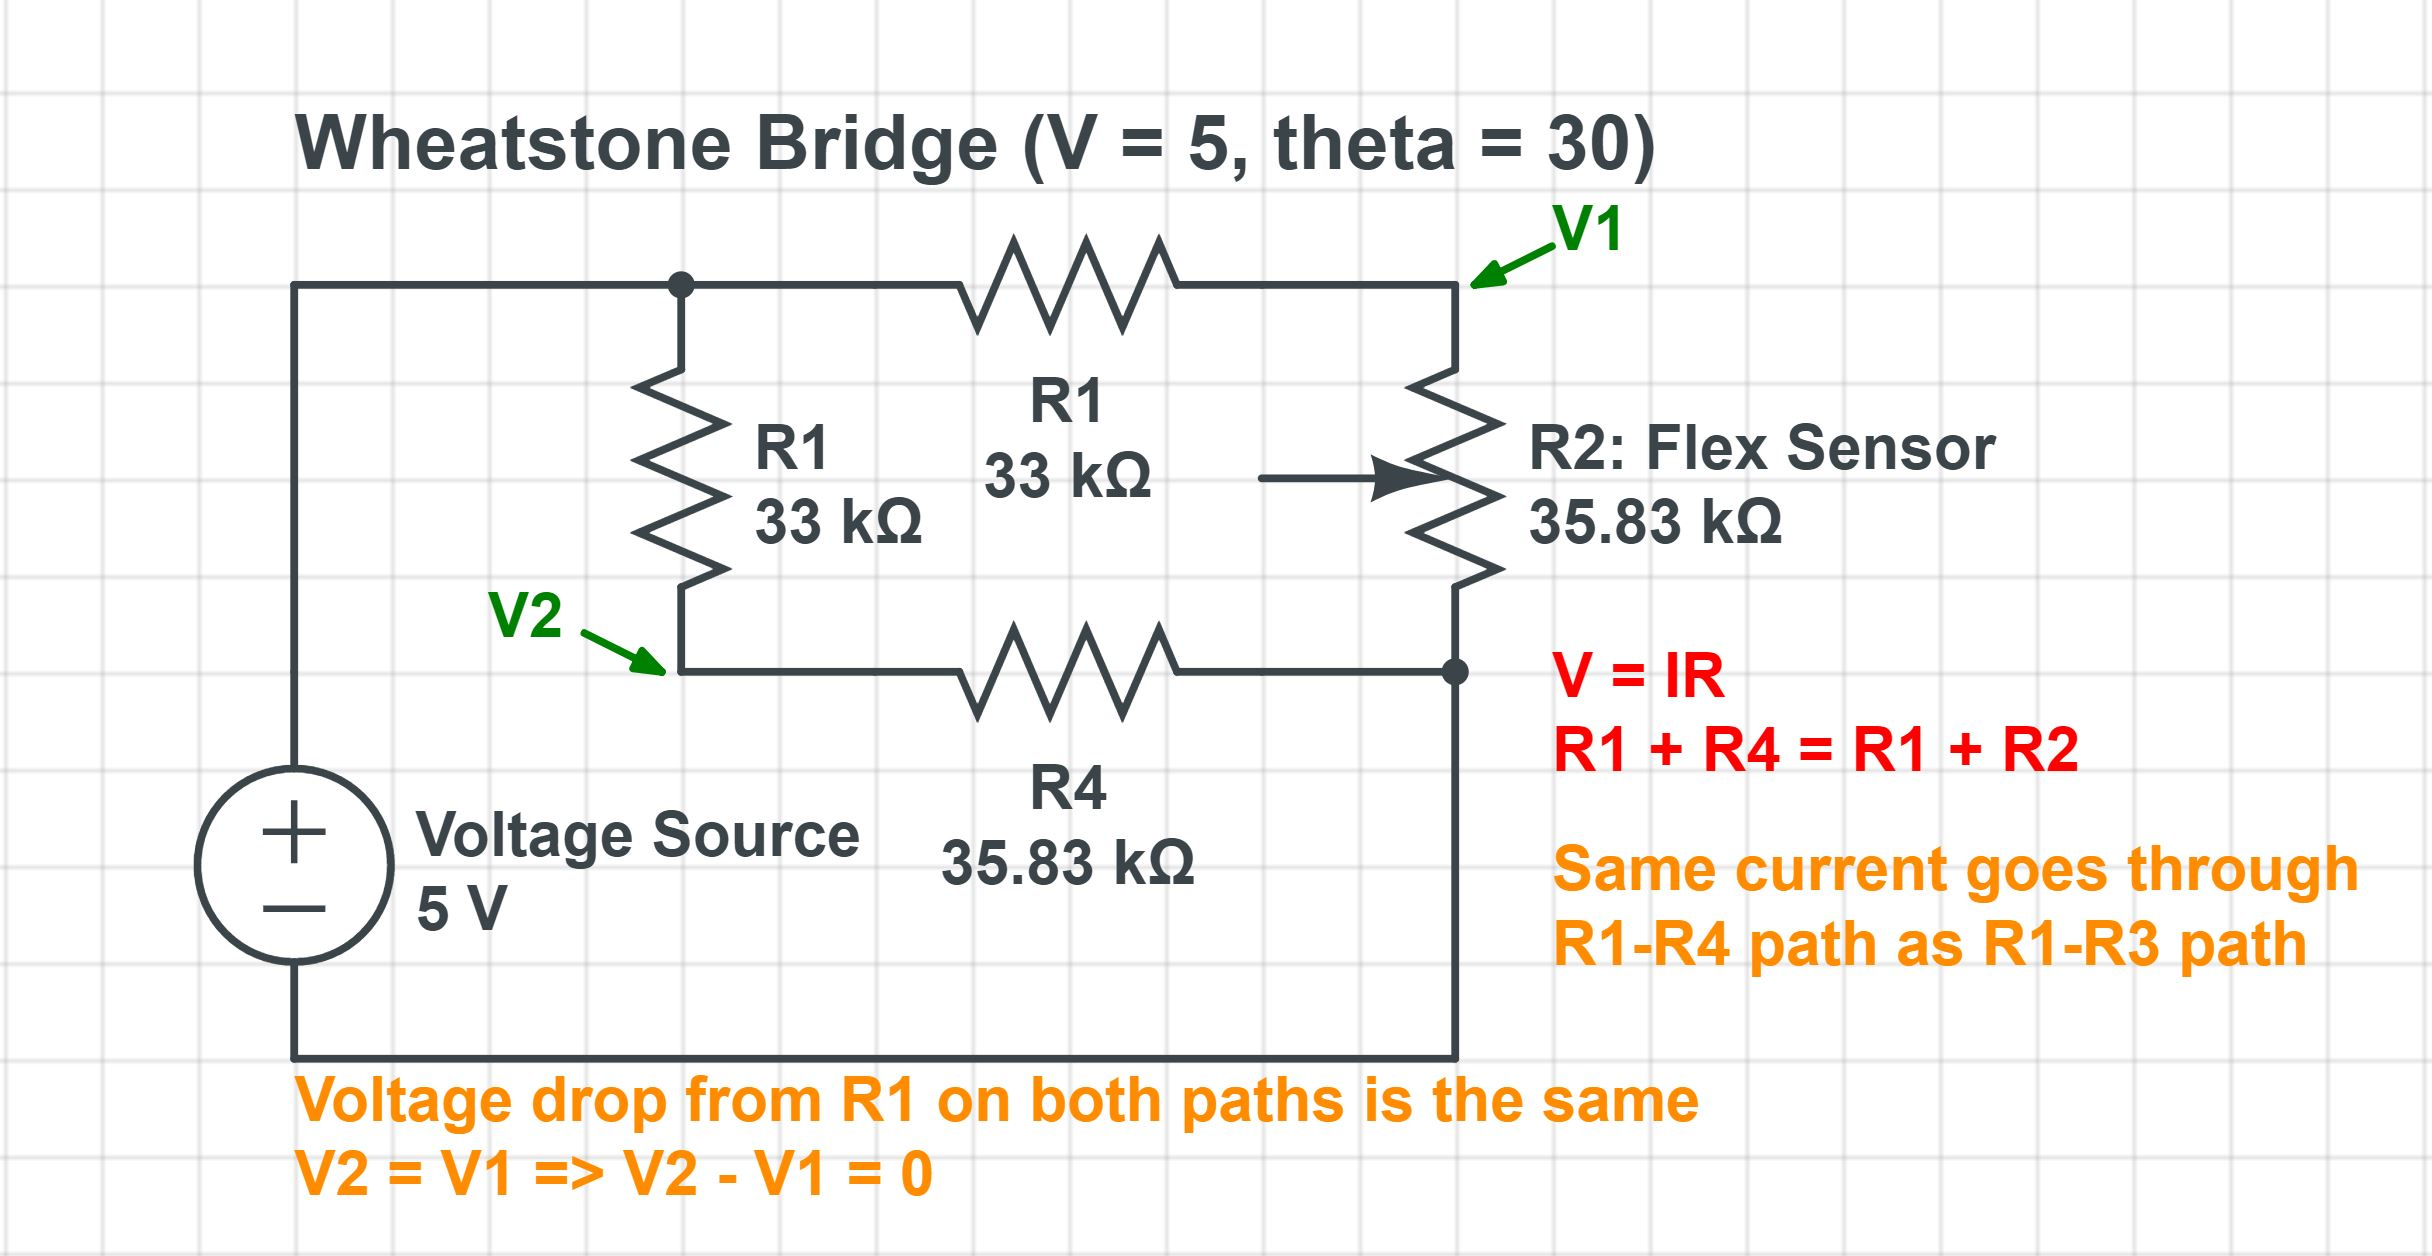
\includegraphics[width=1\textwidth]{inprogress3}
\caption{Wheatstone bridge with $\theta = 30 \degree$ and Voltage Source $ = 5 \ V$}
\end{figure}
\\We see from the diagram that our circuit, the wheatstone bridge, can be represented by two series in parallel, with the input between the two $R_1$s and the ground between $R_2$ and $R_4$. We see that the resistance of each path, the $R_1\to R_4$ path and the $R_1\to R_2$ path, both have the same resistance (which we calculate by addition, since they are in series): $R_{R_1\to R_4} = R_{R_1\to R_2} = 33 + 35.83 = 68.83$. Since both components of the parallel circuit have the same resistance, and voltage is the same across components of a parallel circuits, both components of the parallel circuit  $R_{R_1\to R_4}$ and $R_{R_1\to R_2}$ have the same current $I$.\\ \\
Then, we can calculate the voltage drop by the first element in series by both branches of the parallel circuit by multiplying the resistance of the first element by the current. Since both   $R_{R_1\to R_4}$ and $R_{R_1\to R_2}$ have the same resistor $R_1$ with resistance 33 k$\Omega$, $I \cdot R$ will be the same for both; the voltage drop by the first component of the series for each parallel branch will \textbf{be the same}. We note that this voltage drop will be the same for both branches of the circuit \textbf{regardless of the magnitude of the input voltage}; we see that since we voltage supplied to both branch will be the same regardless of the input voltage, we will have the same voltage drop after the first resistor $R_1$. \\ \\
Then, since we are measuring the remaining voltage at the same point relatively for both branches of the parallel circuit (after the first voltage drop), since they have the same starting voltage, the remaining voltage will be the same as well. Therefore $V_2 = V_1$ so $V_2 - V_1 = 0$V. Once again, this works for \textbf{any} input voltage; since the resistances along the paths are equal, and since the voltage supplied to parallel branches is equal, both paths will have the same voltage drop after $R_1$, regardless of the input voltage amount, resulting in the same remaining $V_1$ and $V_2$ voltages. Therefore $V_2 - V_1 = 0$V.

\end{enumerate}
\pagebreak
\end{document}